\chapter{Results}\label{chap:results}

The analysis will be split into two parts. The first part focuses on the probabilities and frequencies of coincident events, while the second part 
consists of a detailed analysis of the data aquired by the FRT. 

\section{Probabilities of coincident events}\label{sec:muon_coincidence}

When mapping an event rate as a distribution depending on an arbitrary variable, the correlation of the event rate with the corresponding coincident event rate 
within a singular bin, can be approximated as a poisson distribution.
This relation is depicted for different trigger windows in figure~\ref{fig:coin_rate_rate}. 

\begin{figure}
    \centering
    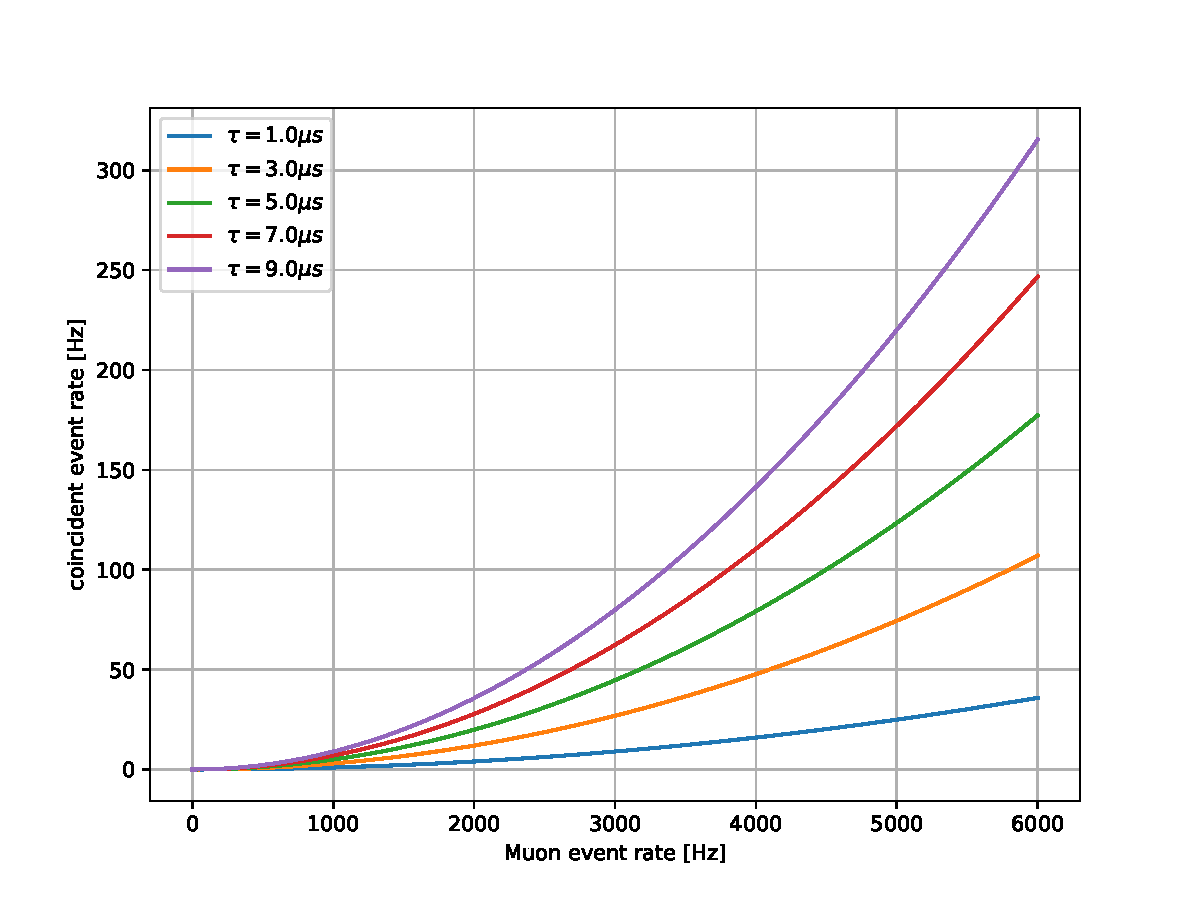
\includegraphics[width=0.7\textwidth]{Plots/coincidence_rate_poisson.pdf}
    \caption{A graph showing the relation between the muon event rate and the corresponding event rate assuming a poisson distributed muon event rate.}
    \label{fig:coin_rate_rate}
\end{figure}

In order to put this into a meaningful context, a relation of the muon event rate and their corresponding energy is extracted from a Monte Carlo simulation, which can 
be found in~\cite{IceProdDataset}.
From this data, a step function $rate(energy)$ can be extracted. Thus, equation~\ref{eq:multi_rate} can be used to visualize the relation between the muon energy and their 
corresponding rate of coincident events. Equivalent calculations are made on a zenith angle spectrum, for which the data is extracted from the same set of monte 
carlo data. Both of these distributions, along with the corresponding intervals, in which the coincidence probability exceeds \SI{0.1}{\percent}, are shown in 
figure~\ref{fig:coin_rate_combined}.

\begin{figure}[ht]
    \centering
    \begin{subfigure}[b]{\textwidth}
        \centering
        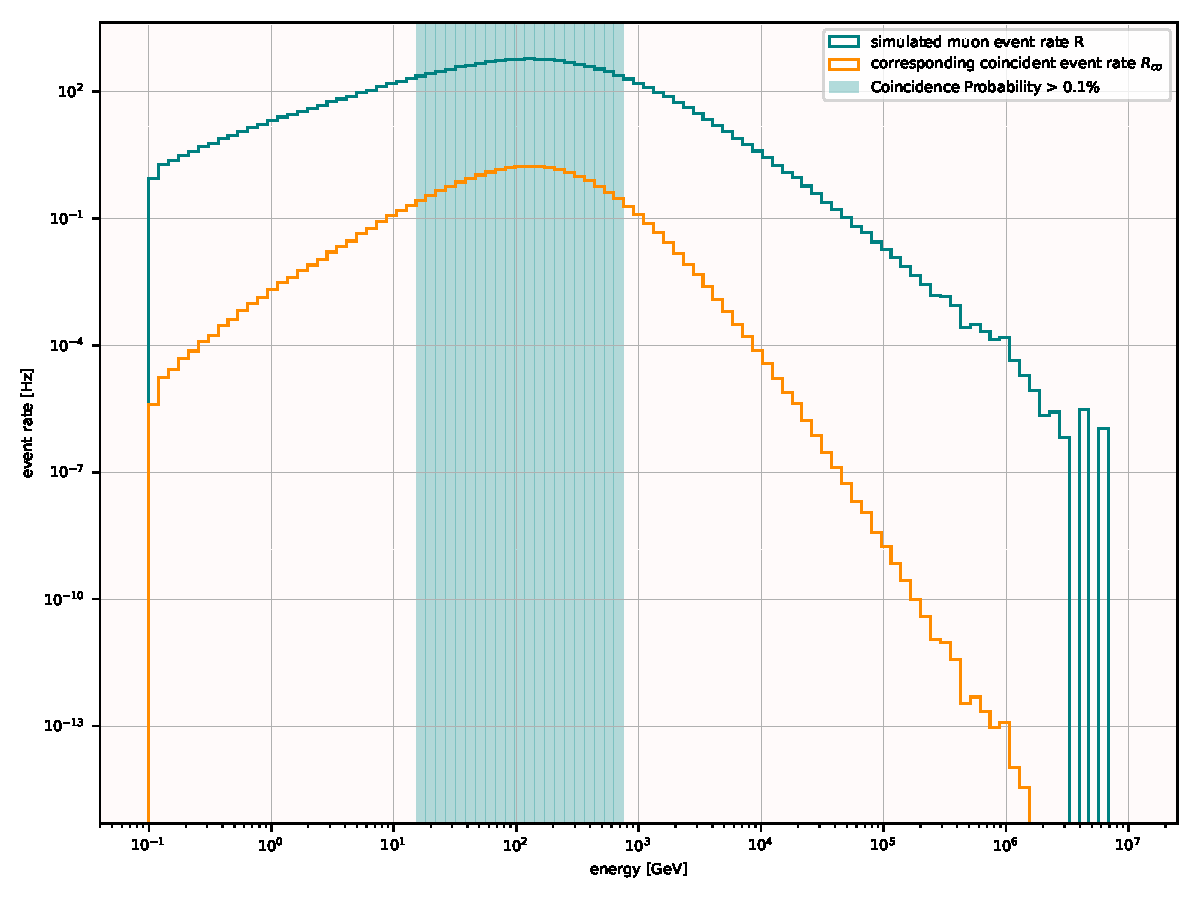
\includegraphics[width=0.7\textwidth]{Plots/coincidence_rate_energy.pdf}
    \end{subfigure}
    \vspace{1em} % Optional vertical space between the plots
    \begin{subfigure}[b]{\textwidth}
        \centering
        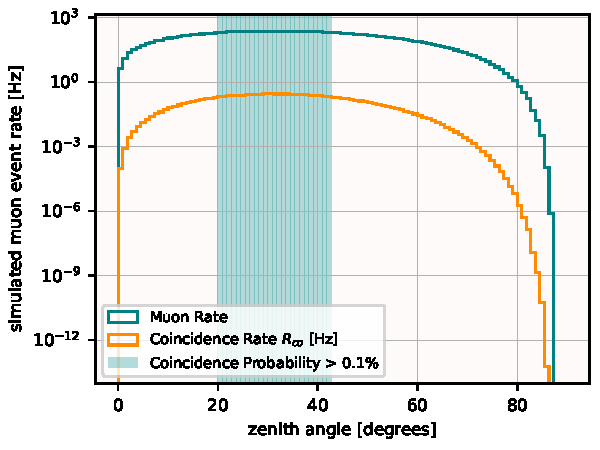
\includegraphics[width=0.7\textwidth]{Plots/coincidence_rate_zenith.pdf}
    \end{subfigure}
    \caption{Comparisons of the muon event rate and corresponding coincident event rate on energy and zenith angle spectra ($\tau = \SI{5}{\micro\second}$)}
    \label{fig:coin_rate_combined}
\end{figure}


Both histograms only show the theoretical coincidence event rate for a fixed trigger window $\tau$. However, different triggers have different readout windows, which 
can significantly change the probability of a coincident event. Treating the readout window as a variable, the coincident event probabilities can be visualized in 
a heat map to get a look at the effects of differing readout windows, as shown in figure~\ref{fig:heatmaps_combined}.

\begin{figure}[ht]
    \centering
    \begin{subfigure}[b]{\textwidth}
        \centering
        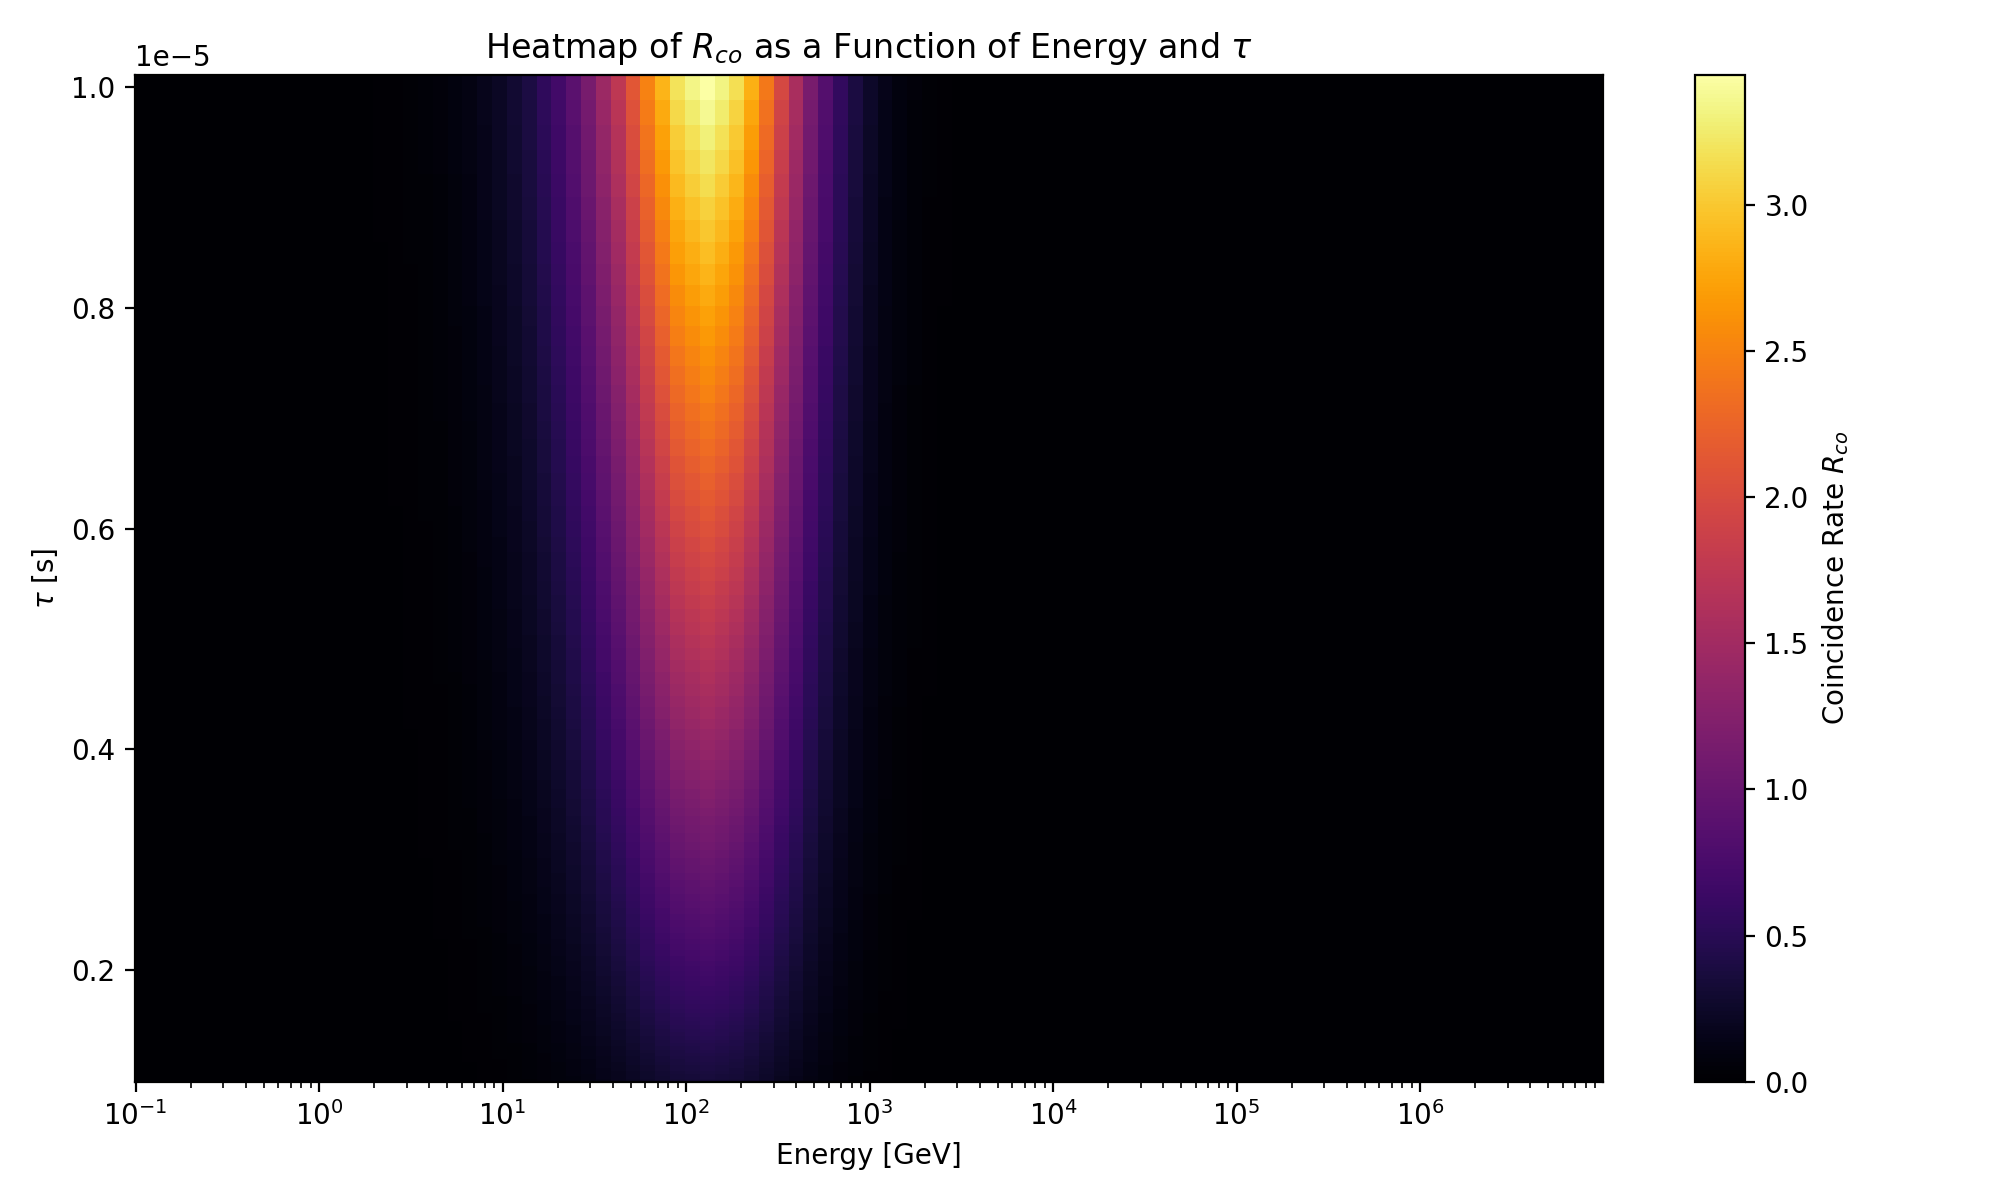
\includegraphics[width=0.7\textwidth]{Plots/heatmap_energy.png}
    \end{subfigure}
    \vspace{1em} % Optional vertical space between the plots
    \begin{subfigure}[b]{\textwidth}
        \centering
        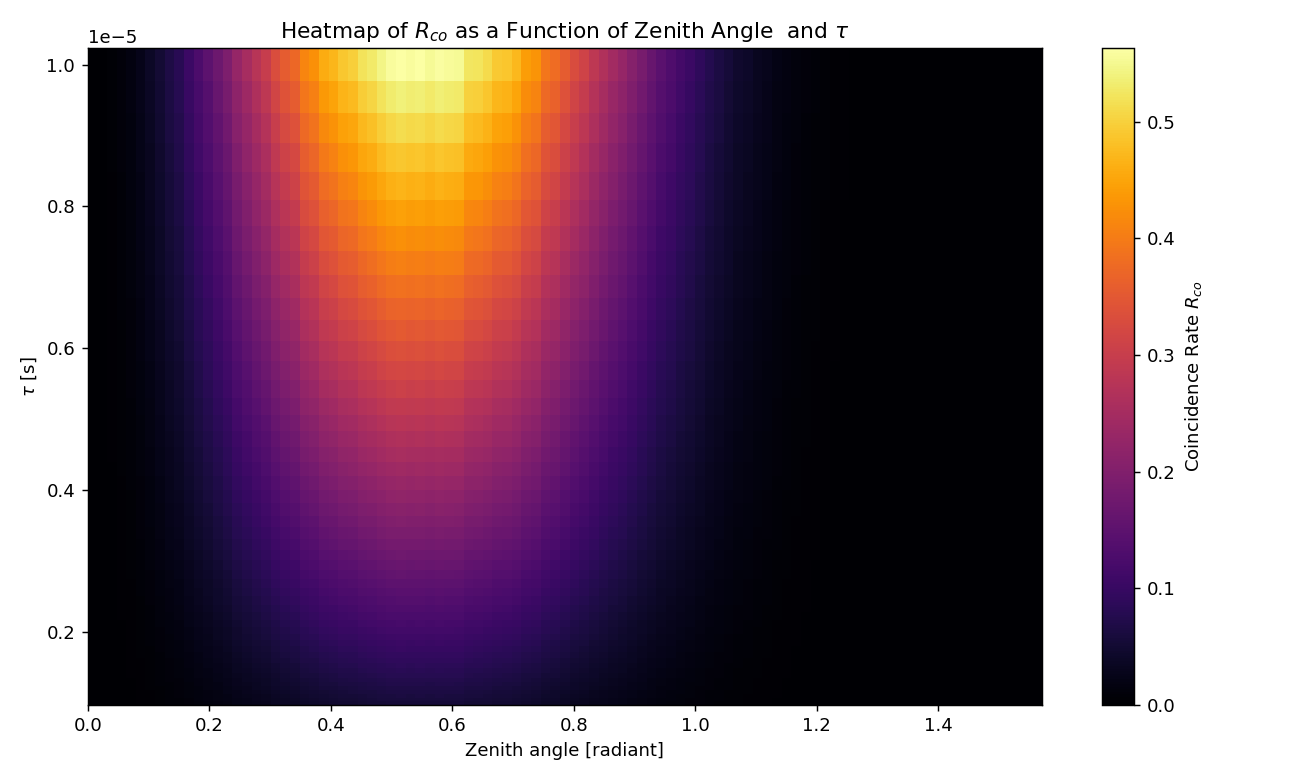
\includegraphics[width=0.7\textwidth]{Plots/heatmap_zenith.png}
    \end{subfigure}
    \caption{Prototypes of the heatmaps for energy and zenith angle spectra.}
    \label{fig:heatmaps_combined}
\end{figure}

\section{Analysis of the Fixed Rate Trigger}

As mentioned in section~\ref{sec:daq}, the FRT has a comparatively large readout window of \SI{10}{ms}. The result of this is that one \textit{event} contains 
a substantial amount of DOM hits. Since the average muon rate in IceCube is around \num{2200}\unit{Hz}, there is a considerable likelihood, that any \textit{event}
contains physically significant signals. Other than muon events, there might be neutrino events as well as other possible atmospheric or astrophysical signals 
being measured in a given readout window of the FRT. However, a major fraction of the signals detected by the FRT is expected to be noise. 
The subsequent analysis is an attempt to extract knowledge about the composition of the signals 
measured by the FRT and to possibly use them to better understand coincident events in IceCube. All of the subsequent analyses are created using the 'FRT only' dataset~\cite{IceCubeFRT} 
from the entirety of May 2016. \\

The first step breaking down the FRT's data is to inspect the kind of signals detected in a singular DOM hit. In accordance with the description of 
\textit{subevents} in \ref{sec:daq}, the relevant signals are filtered out. Depicted in 
figure~\ref{fig:frt_mu_sub_comp_1} is a comparison of the unfiltered versus filtered signals detected over the course of \num{5035} \textit{events}. 
When referring to an \textit{event} of the FRT, it denotes a complete readout window containing the detected signals. Also, wherever something is labeled as filtered, 
it means the signals are part of the \textit{subevents}
Most notably, the two distributions show a 
general similarity between them. As expected, there are substantially more unfiltered signals than filtered signals. This shows that there are in fact signals 
being filtered. The expectation would be to see a clear shift towards higher 
charge values in distribution of filtered signals, based on the idea that signals which stem from astrophysical or atmospheric sources would carry higher energy 
than noise signals. The observation does not quite match this expectation of clearly distinguished distributions. 

\begin{figure}[H]
    \centering
    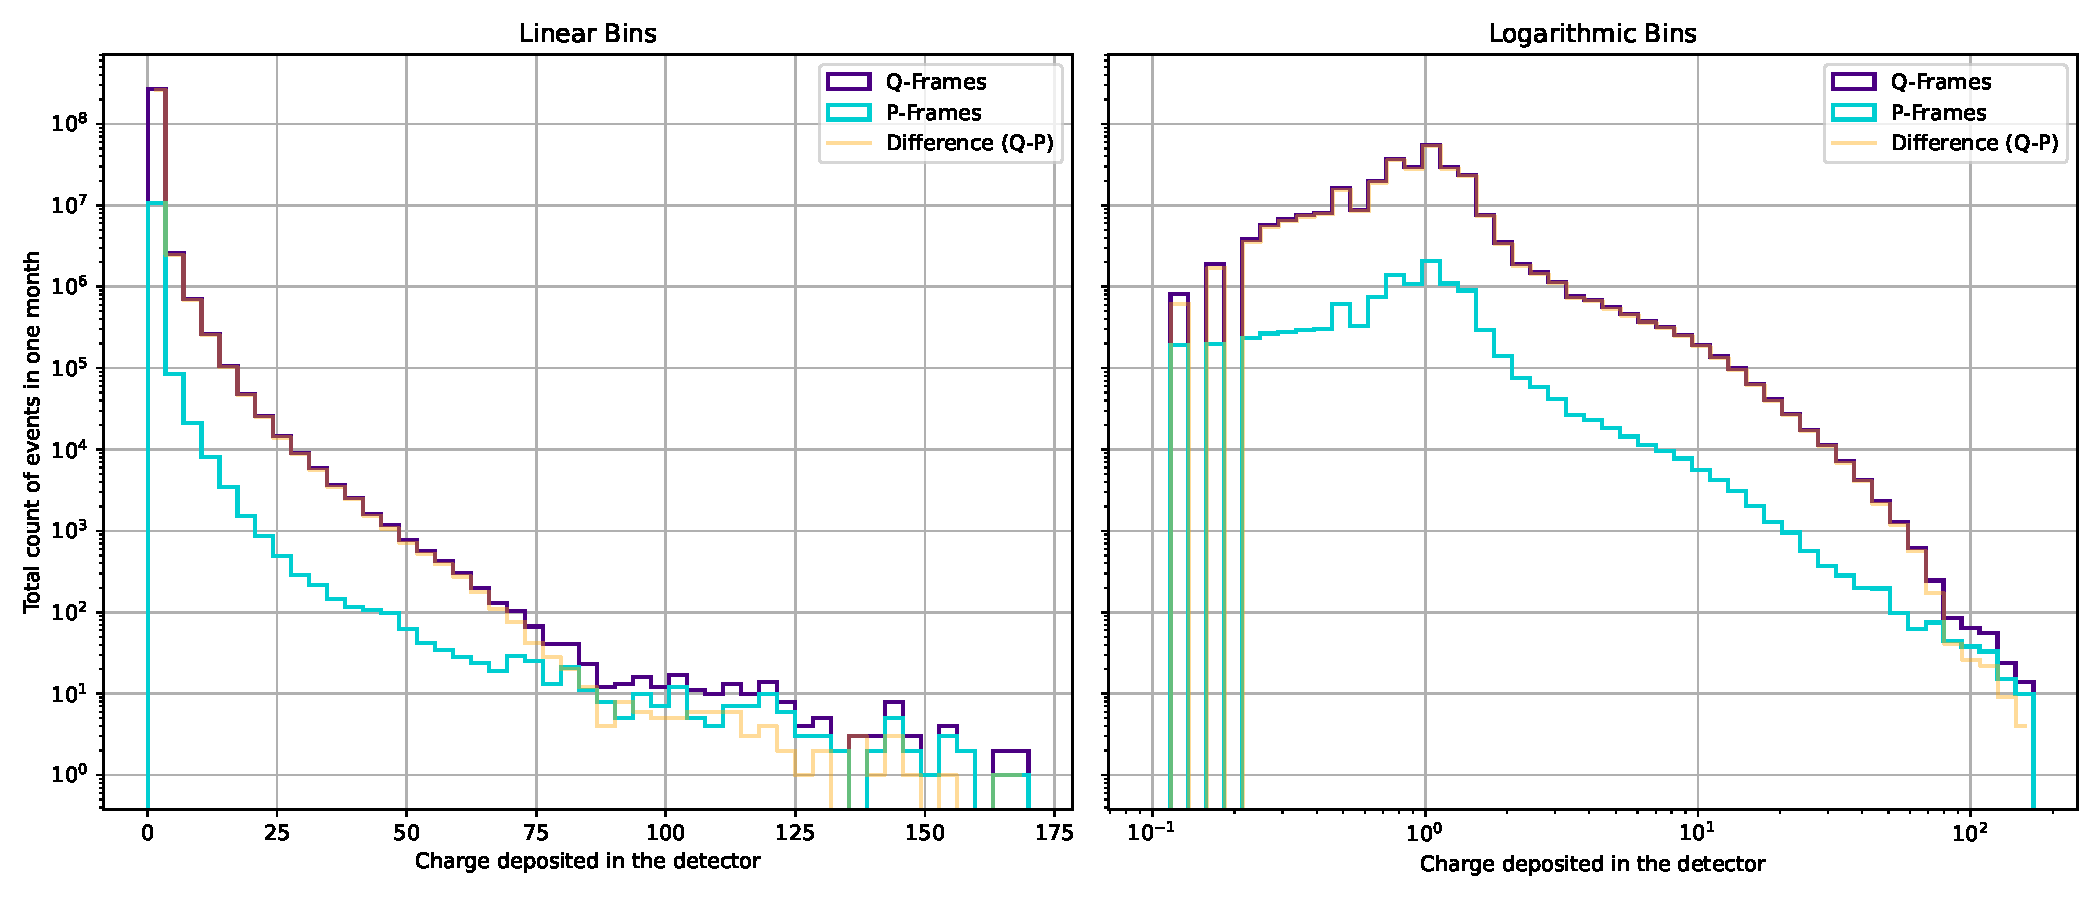
\includegraphics[width=\textwidth]{Plots/q_p_comp.pdf}
    \caption{A comparison between the counts of all Signals and physics signals.}
    \label{fig:frt_mu_sub_comp_1}
\end{figure}

To gather a deeper understanding of the signals measured and how they might be filtered, a comparison of mean charges for the individual DOMs is created. 
Figure~\ref{fig:mean_dom_charge_pq} shows the mean charge per DOM hit of every individual DOM over \num{5035} \textit{events}. In the following, the individual DOMs 
are identified by their 'string'- and 'om' id respectively.
The mean charges are quite evenly distributed throughout the DOMs, with the exeption of the DOM (61,13), which shows an unusually high mean charge of 
\num{5.08}~\unit(PE). Another notable characteristic of the filtered signals, although not easily visible, is the slightly higher mean charge around the 35th om. 
%(values)
Other than that, there are no immediately visible anomalies in the general pattern of mean charges throughout the detector. 

\begin{figure}[H]
    \centering
    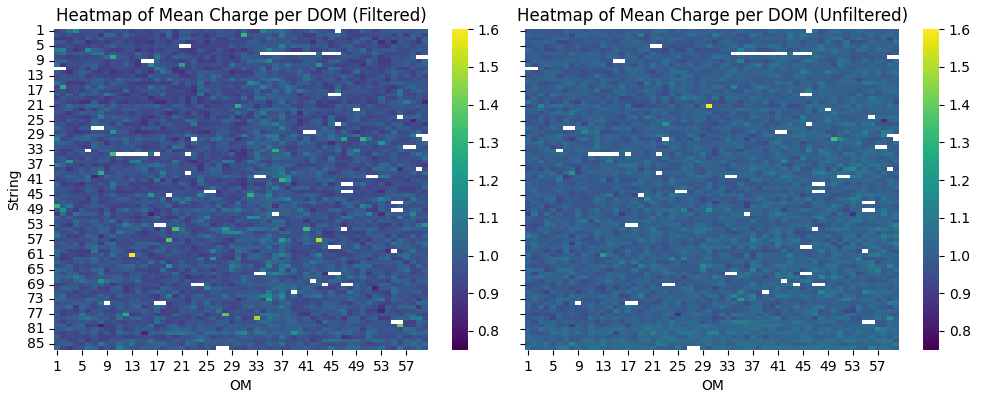
\includegraphics[width=\textwidth]{Plots/mean_charge_all_dom.png}
    \caption{The mean charge of every individual DOM for filtered and unfiltered signals.}
    \label{fig:mean_dom_charge_pq}
\end{figure}

While the analysis of mean charges over time allow for the possible detection of general anomalies or trends across the DOMs, it does not provide clear indicators for 
significant signals without additional information. When detecting a substantial signal, the expected behavior is a clear spike in the charge over time function. 
Measuring these signals frequently might therefore have a visible impact on the standard deviation of the measured charge. The comparison of filtered and unfiltered 
signals regarding the mean charge values and their standard deviation is shown in figure~\ref{fig:mean_std_comp}.

\begin{figure}[H]
    \centering
    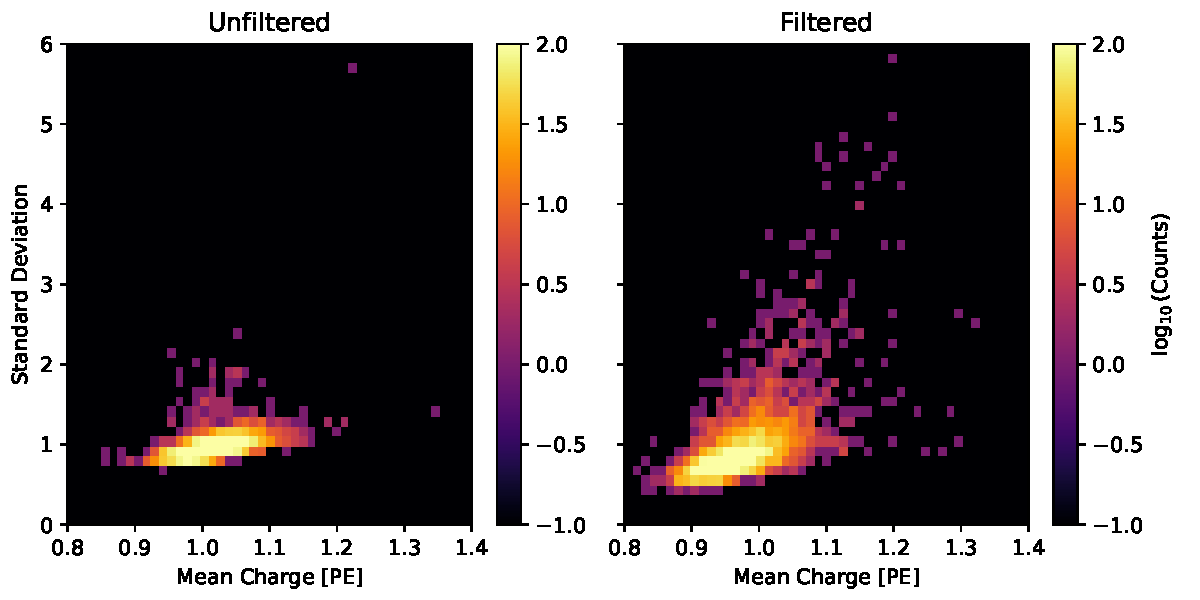
\includegraphics[width=0.9\textwidth]{Plots/mean_std_charge.pdf}
    \caption{A Comparison of the mean charge and standard deviation for filtered and unfiltered signals.}
    \label{fig:mean_std_comp}
\end{figure}

Clearly visible is the substantially larger spread of charges in the filtered signals. While the mean charges do not differ significantly from those of the 
unfiltered signals, there is a notable tendency towards larger deviation from the mean charge for the filtered signals. 
On the one hand, this tendency suggests multiple measurements of high energy signals in those DOMs which show these high standard variations. On the other hand,
the observation that the vast 
majority of filtered signals are clustered around a similar mean charge and standard deviation, as seen in figure~\ref{fig:mean_std_hist}, leads to the speculation 
that the filtered signals might still contain a considerable amount of noise.

\begin{figure}[H]
    \centering
    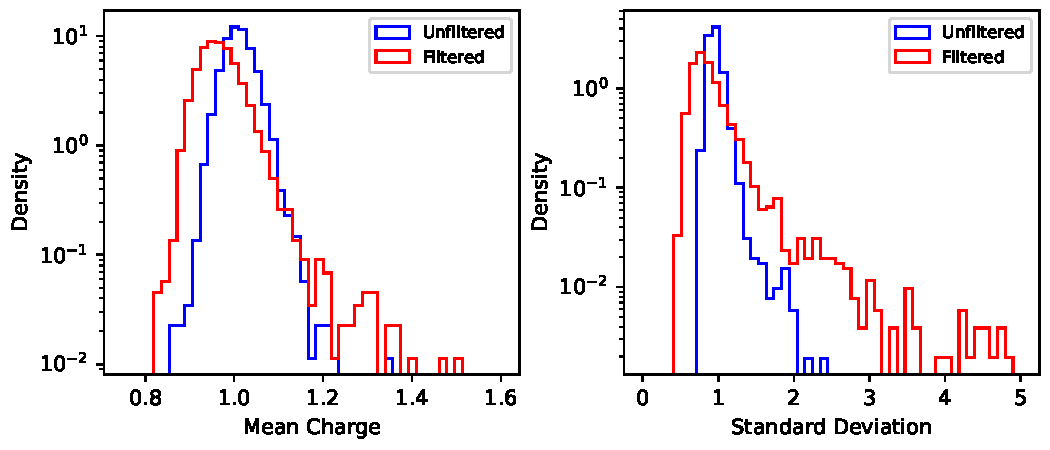
\includegraphics[width=0.9\textwidth]{Plots/qp_mean_std_comparison_histograms.pdf}
    \caption{An Individual Comparison of the mean charge and standard deviation.}
    \label{fig:mean_std_hist}
\end{figure}

Another interpretation could be, that the majority of signals of interest have infact comparatively low energies, leading to an average charge per DOM hit of 
just below \num{1}~\unit{PE}. A disirable characteristic to observe would have been a certain charge threshold, below which none of the filtered signals 
would be observed. This would result in a strict condition that could be applied to certain triggers or other software. However, this is not the case. 


% further analysis:
% 1. charge over time p and q
% 2. charge over time in single events
% 3. filtermask with different plots
% 4. filter event candidates via simple algorithm -> clusters

Thus far, the signals detected by the FRT have been analyzed with a focus on individual DOM behavior. While this insight on the difference between filtered and 
unfiltered events is generally interesting, it does not provide any direct information, that could be used for the analysis of coincident events. Therefore, further 
characteristics are inspected, with the aim of finding certain properties, which might characterize possible coincident events.

The first unexplored property to examine is the charge per 
time function within singular events. Since one event accompasses a time window of \SI{10}{\milli\second}, a significant number of signals should be 
recorded for one event. This charge distribution over time for the entire detector is shown in figure~\ref{fig:charge_time_1}, once on a logarithmic scale to show 
the entire charge spectrum, and once on a linear scale around the mean charge, visualizing the variance more intuitively. 

\begin{figure}[ht]
    \centering
    \begin{subfigure}[b]{\textwidth}
        \centering
        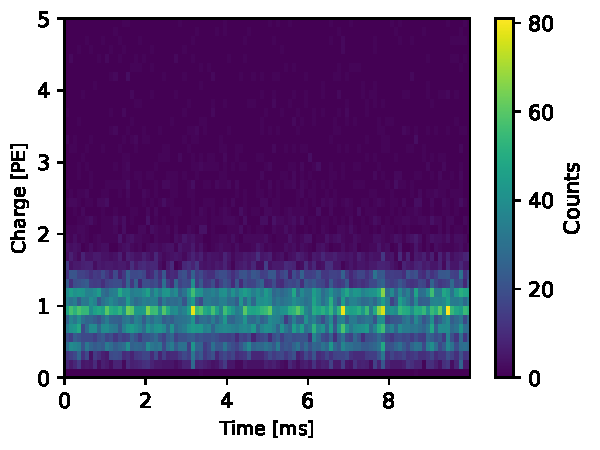
\includegraphics[width=0.7\textwidth]{Plots/charge_time_1_lin.pdf}
    \end{subfigure}
    \vspace{1em} % Optional vertical space between the plots
    \begin{subfigure}[b]{\textwidth}
        \centering
        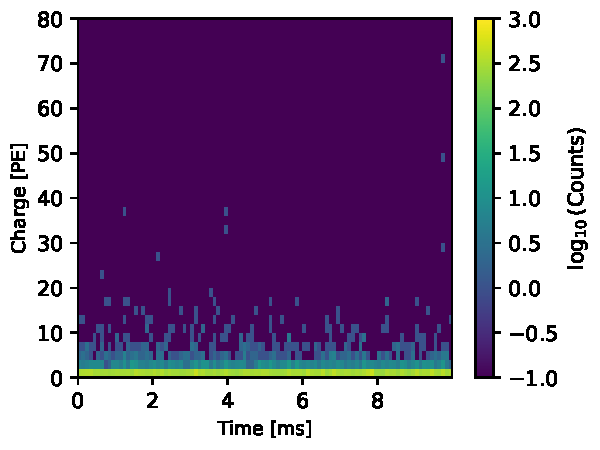
\includegraphics[width=0.7\textwidth]{Plots/charge_time_1_log.pdf}
    \end{subfigure}
    \caption{charge per time within one event (entire detector).}
    \label{fig:charge_time_1}
\end{figure}

Due to the long readout window of the FRT, the charge per time function shows no notable characteristics at this scale. Neither does it differ significantly between 
individual events. This leads back to the inspection of the filtered signals. These signals are clustered in subevents, which should have significantly
more distinct features with regards to their corresponding charge over time measurements. From the previous analysis however, these filtered subevents 
have been demonstrated to contain a substantial amount of signals with comparatively low charges. As a visual comparison, three subevents with comparatively high 
total charges are shown next to three average subevents. 

\begin{figure}[H]
    \centering
    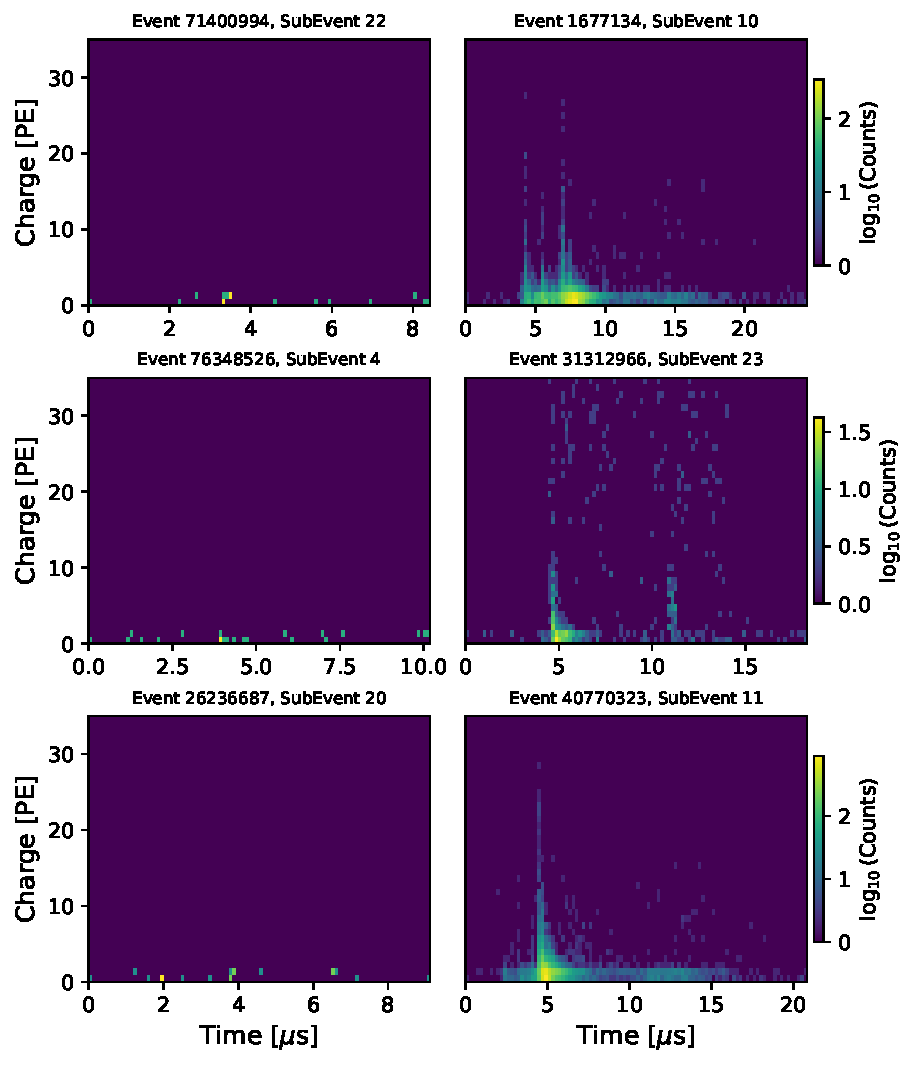
\includegraphics[width=0.9\textwidth]{Plots/heatmaps_lowest_highest_charge_subevents.pdf}
    \caption{Comparison of Subevents with Charges of different Magnitudes (high charges on the right, low charges on the left).}
    \label{fig:high_low_comp}
\end{figure}
% \begin{figure}[h!]
%     \centering
%     % First row
%     \begin{subfigure}[t]{0.49\textwidth}
%         \centering
%         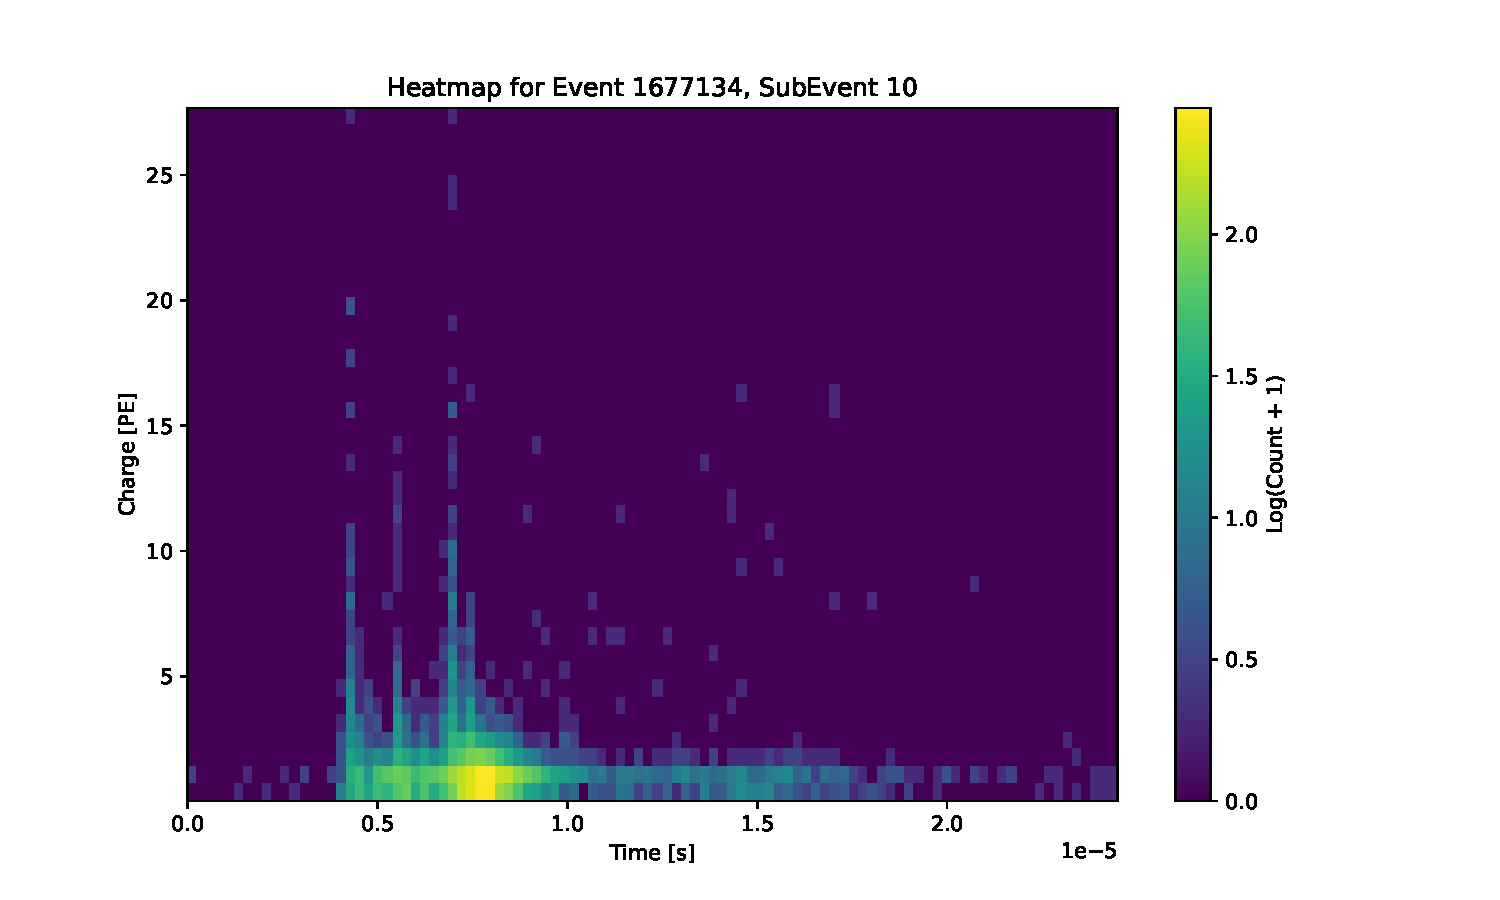
\includegraphics[width=\textwidth]{Plots/heatmap_subevent_triple_high.pdf}
%         \caption{SubEvent 1: Description here.}
%         \label{fig:subevent1}
%     \end{subfigure}
%     \hfill
%     \begin{subfigure}[t]{0.49\textwidth}
%         \centering
%         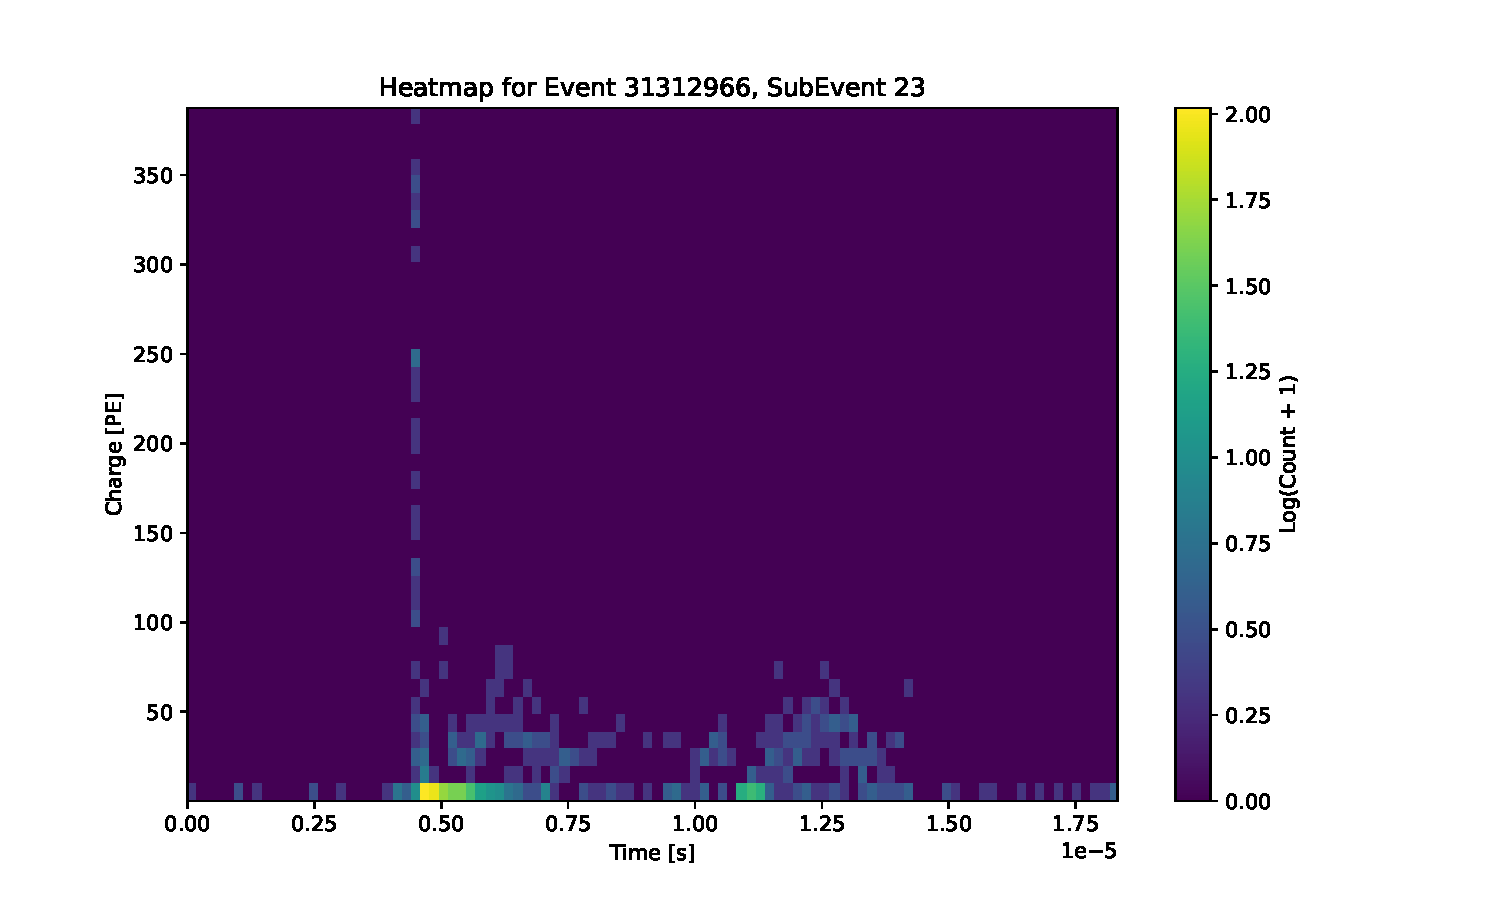
\includegraphics[width=\textwidth]{Plots/heatmap_subevent_double_high.pdf}
%         \caption{SubEvent 2: Description here.}
%         \label{fig:subevent2}
%     \end{subfigure}
    
%     % Second row
%     \vspace{0.5cm} % Adjust vertical spacing as needed
%     \begin{subfigure}[t]{0.49\textwidth}
%         \centering
%         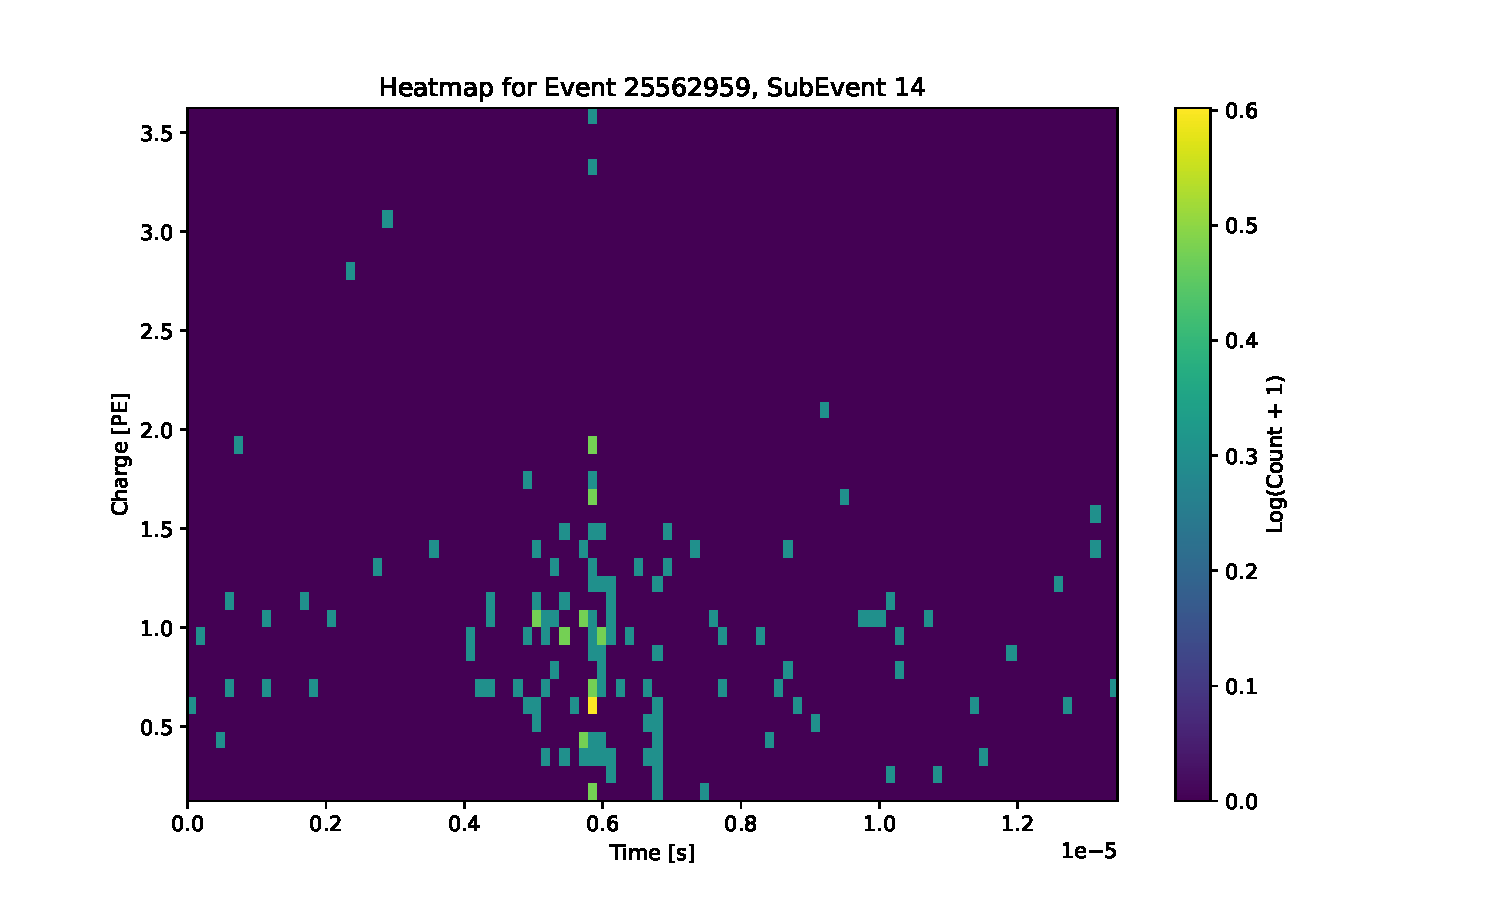
\includegraphics[width=\textwidth]{Plots/heatmap_subevent_random_1.pdf}
%         \caption{SubEvent 3: Description here.}
%         \label{fig:subevent3}
%     \end{subfigure}
%     \hfill
%     \begin{subfigure}[t]{0.49\textwidth}
%         \centering
%         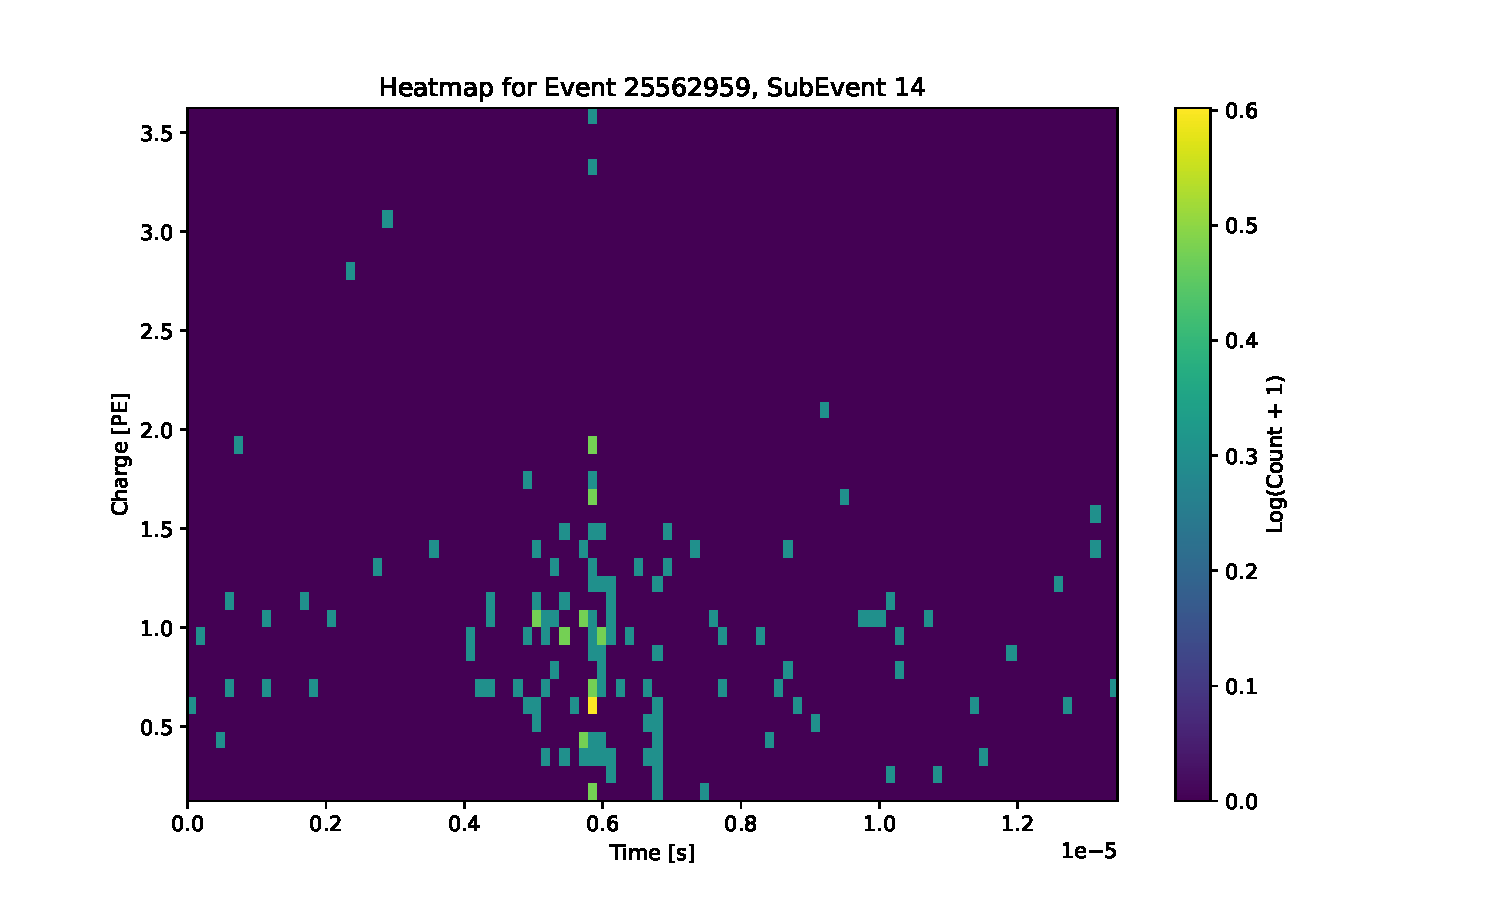
\includegraphics[width=\textwidth]{Plots/heatmap_subevent_random_1.pdf}
%         \caption{SubEvent 4: Description here.}
%         \label{fig:subevent4}
%     \end{subfigure}

%     % Main caption for the figure
%     \caption{Comparison of heatmaps for four different SubEvents. }
%     \label{fig:subevent_charge_time}
% \end{figure}


While the visual difference between these subevents of vastly differing mean charge is immediately evident, a specificly interesting characteristic can be 
observed for the subevents on the upper right and on the center right. These subevents show multiple peaks of charge and signal count within their individual time frame. As these features
might be indicators for coincident events, these structures are analyzed in detail. 

Disclaimer for the following analysis: \\
determining coincident events with significant certainty requires complex methods, exceeding the scope of this thesis. For this reason, an approach is adopted that may 
not directly identify which subevents contain coincident events but can narrow down the potential candidates for such events. this approach is to find clusters of 
high charge and high signal counts within each subevent, with the aim of finding subevents with a multitude of such clusters. While a muon for example could deposit 
energy at multiple points in time while crossing the detector, leading to multiple peak also, a subevent with a single cluster is highly unlikely to contain multiple
events. 
In the subsequent analysis, the python function $\text{find\_peaks}$ from 
the scipy library is used. Singular events are characterized by a combination of the charge values, as well as the signal counts on a time scale within the time 
frame of a subevent. This time frame is divided into \num{100} equally spaced bins. For each bin, the sum of the charges ($Q_P$) measured within is calculated, 
as well as the total counts ($N_P$) within in the bin. These projections are combined into a weighted projection ($W_P$)

\begin{equation}
    W_P = \alpha\cdot Q_P +  \beta\cdot N_P\,
\end{equation}

where the weights \alpha and \beta are calculated via the equation

\begin{align}
    \alpha &= \frac{M_N + \sigma_N^2}{(M_C + \sigma_C^2) + (M_N + \sigma_N^2)} \\
    \beta &= 2\frac{M_C + \sigma_C^2}{(M_C + \sigma_C^2) + (M_N + \sigma_N^2)}
\end{align}


where $(M_C)$ and ($M_N$) represent the sums of the charge and count projections, respectively, and ($\sigma_C^2$) and ($\sigma_N^2$) denote their variances. 
These weights ensure that both the magnitude and variability of the projections are accounted for in the weighted projection. 

$W_P$ is then used as the function for which the $\text{find\_peaks}$ method is applied. This method takes multiple parameters, which were determined empirically 
based on a variety of subevent samples. These parameters are shown in table~\ref{tab:peak_parameters} along with their respective description.


\begin{table}[h!]
    \centering
    \caption{Final parameters used for peak detection in the weighted projection of charge and count data.}
    \begin{tabular}{|l|l|p{7cm}|}
    \hline
    \textbf{Parameter} & \textbf{Value} & \textbf{Description} \\ \hline
    Prominence & 5 & The minimum vertical distance a peak must stand out relative to its neighboring valleys. This ensures that only significant peaks are detected. \\ \hline
    Height & Dynamic (\(5\%\) baseline + \(1.5 \cdot \sigma\)) & The minimum value a peak must reach to be considered valid. This threshold is calculated dynamically based on the signal's baseline noise (5th percentile) and its standard deviation (\(\sigma\)). \\ \hline
    Distance & 4 bins & The minimum number of bins required between consecutive peaks to ensure they are sufficiently separated and not falsely grouped. \\ \hline
    \end{tabular}
    \label{tab:peak_parameters}
\end{table}


The workings of this method are visualized for an example subevent in figure~\ref{fig:find_peaks}

\begin{figure}[ht]
    \centering
    \begin{subfigure}[b]{\textwidth}
        \centering
        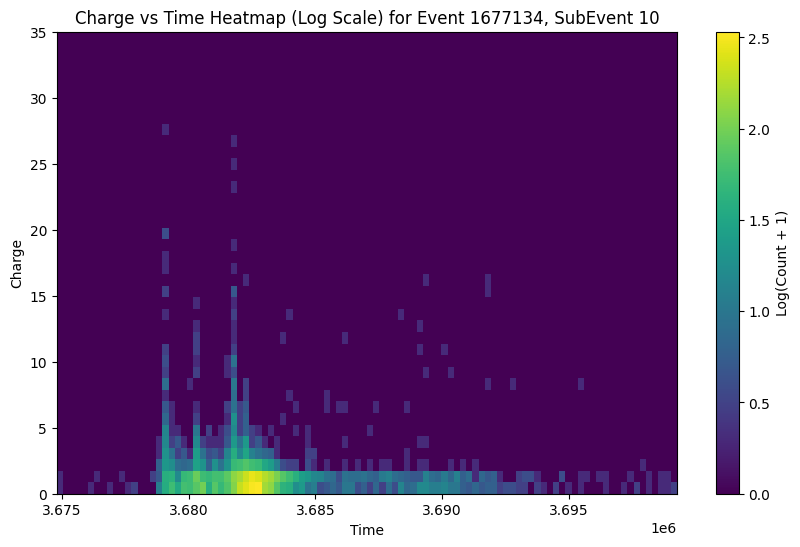
\includegraphics[width=0.7\textwidth]{Plots/peak_heat_1.pdf.png}
    \end{subfigure}
    \vspace{1em} % Optional vertical space between the plots
    \begin{subfigure}[b]{\textwidth}
        \centering
        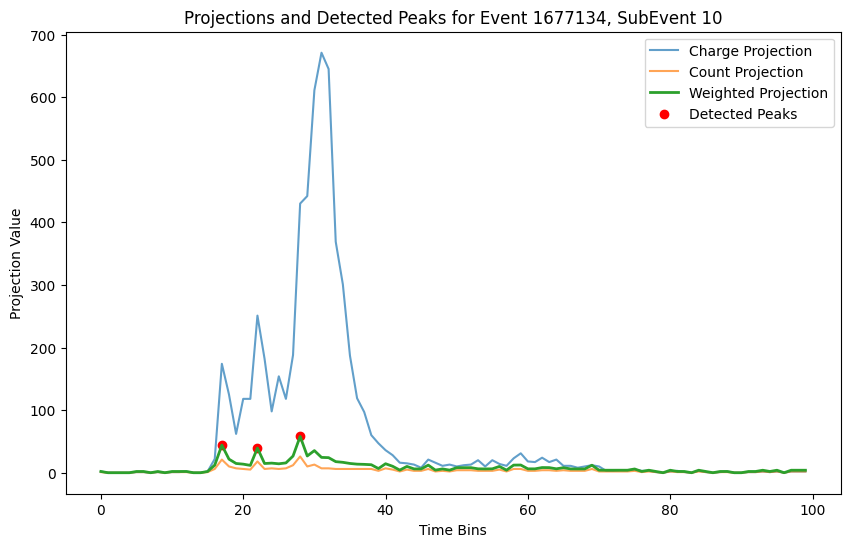
\includegraphics[width=0.7\textwidth]{Plots/peak_plot_1.png}
    \end{subfigure}
    \caption{Charge per Time heatmap for an example Subevent along with a depiction of the associated peak finding method.}
    \label{fig:find_peaks}
\end{figure}

These are the results from the implemented method:
\begin{align}
    \text{Total subevents} &= 137342 \\
    \frac{N(\text{multiple peaks})}{N(\text{any peaks})} &= 0.54 \\
    \frac{N(\text{any peaks})}{N(\text{total})} &= 0.85
\end{align}

The evaluation of these results is discussed in the subsequent chapter~\ref{chap:discussion}










